\documentclass[utf8]{article}
\usepackage{amsmath,amssymb}
\usepackage{graphicx}
\usepackage{fullpage}
\usepackage{setspace}
\usepackage{verbatim}

\usepackage{algorithm}
\usepackage{algorithm}
\usepackage{algorithmicx}
\usepackage{algpseudocode}
\usepackage{amsmath}
\usepackage{subfigure}
\usepackage[top=2cm, bottom=2cm, left=2cm, right=2cm]{geometry}

\onehalfspacing

\title{\bf\huge Lab3 Design Document}
\author{Mei Yixuan 2019011041 Yao92}
\date{\today}

\renewcommand{\algorithmicrequire}{\textbf{Input:}}  
\renewcommand{\algorithmicensure}{\textbf{Output:}} 

\begin{document}
\maketitle

\section{Advanced Cache Replacement Policies}

\subsection{LRU-LIP}
In LRU-LIP, we set counter of the newly inserted block as the number of valid ways in the corresponding set minus one. This ensures that newly added blocks are in the least important position. Also, the counters are continuous (i.e. if we have 3 valids ways, their counters have value 0, 1 and 2). This nice property makes eviction and reversion much easier: we can simply use the same function as in LRU. The hardware control overhead of LRU-LIP is one counter each way, which is identical to LRU. Exact hardware cost is in the following figure.
\begin{figure}[h]
	\centering
	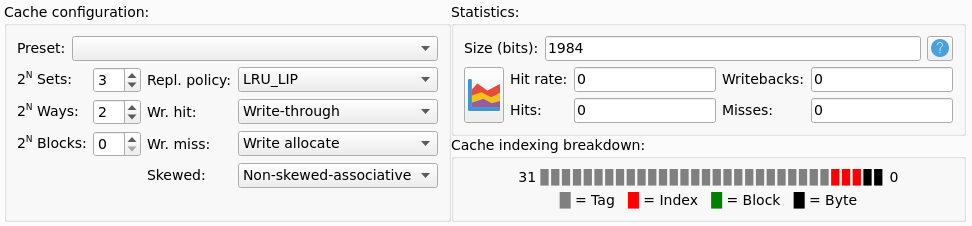
\includegraphics[width=0.7\linewidth]{screenshot001}
	\caption{LRU-LIP Hardware Cost}
	\label{fig:screenshot001}
\end{figure}


\subsection{DIP}
In DIP, we use the first set (SET0) as MIP sample and the second set (SET1) as LIP sample. In each memory access on non-dueling sets (i.e. sets other than SET0 and SET1), we update cache control fields according to current better replacement policy. We reset all counters every 100000 memory accesses to avoid potential risk of overflow. Thanks to the good property of LRU-LIP, eviction and reversion of DIP is also identical to LRU. Besides the counter in each way, DIP also needs five counters for data recording. Exact hardware cost is in the following figure.
\begin{figure}[h]
	\centering
	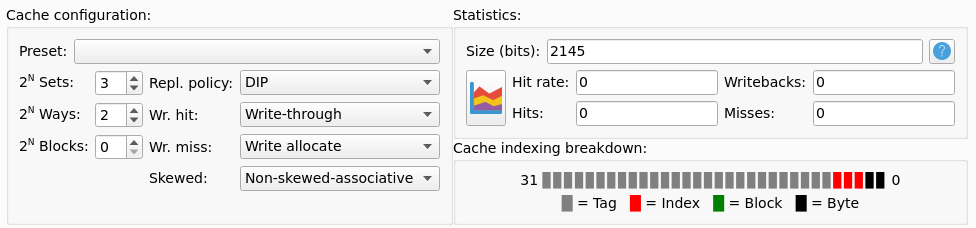
\includegraphics[width=0.7\linewidth]{screenshot002}
	\caption{DIP Hardware Cost}
	\label{fig:screenshot002}
\end{figure}
\newpage

\subsection{RRIP}
In RRIP, we use counter field of each way to store its RRI. It has field width of 3 bits. Upon hit, we set RRI of corresponding entry as 0. Upon insertion, we set RRI of corresponding entry as long RRI (i.e. 6). When choosing a block for eviction when all ways are occupied, we choose the block with largest RRI and normalize all values to distant RRI (this is identical to adding one repeatedly). Exact hardware cost is in the following figure.
\begin{figure}[h]
	\centering
	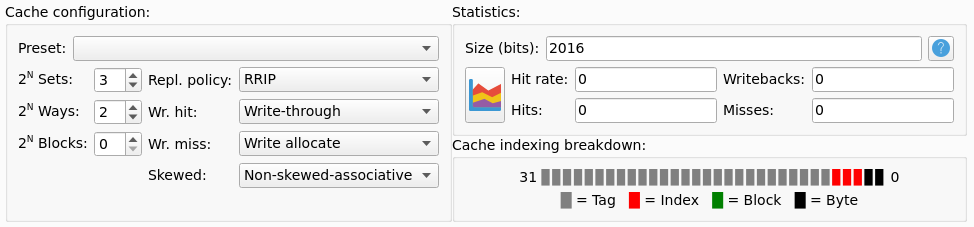
\includegraphics[width=0.7\linewidth]{screenshot003}
	\caption{RRIP Hardware Cost}
	\label{fig:screenshot003}
\end{figure}

\subsection{Results}
Results of different replacement policies:
\newline

\resizebox{\textwidth}{18mm}{
\begin{tabular}{|c|c|c|c|c|}
		\hline
		Design & Benchmark 1 Miss Rate & Benchmark 2 Miss Rate & Benchmark 1 Total Cycles & Benchmark 2 Total Cycles \\
		\hline
		No Cache & 100 & 100 & 2083191 & 23508468 \\
		\hline
		Random Replacement & 16.47 & 2.44 & 1230758 & 9275269 \\
		\hline
		LRU Replacement & 13.86 & 1.99 & 1204202 & 9209763 \\
		\hline
		LRU-LIP Replacement & 14.77 & 2.76 & 1213470 & 9322490 \\
		\hline
		DIP-Replacement & 14.66 & 2.27 & 1212268 & 9250427 \\
		\hline
		RRIP-Replacement & 13.71 & 2.24 & 1202611 & 9246016 \\
		\hline
\end{tabular}}
\newline

\noindent
Results of different cache capacities and mapping schemes:
\newline

\resizebox{\textwidth}{33mm}{
\begin{tabular}{|c|c|c|c|c|}
	\hline
	Capacity and Mapping & Benchmark 1 Miss Rate & Benchmark 2 Miss Rate & Benchmark 1 Total Cycles & Benchmark 2 Total Cycles \\
	\hline
	16-entry direct-mapped & 29.71 & 26.23 & 1365868 & 12745909 \\
	\hline
	16-entry 4-way associative & 28.74 & 7.52 & 1356019 & 10016283 \\
	\hline
	16-entry 8-way associative & 29.67 & 3.56 & 1365525 & 9439026 \\
	\hline
	16-entry fully-associative & 30.32 & 3.53 & 1372080 & 9433830 \\
	\hline
	32-entry direct-mapped & 19.01 & 19.73 & 1256732 & 11798043 \\
	\hline
	32-entry 4-way associative & 13.86 & 1.99 & 1204202 & 9209763 \\
	\hline
	32-entry 8-way associative & 12.72 & 1.92 & 1192565 & 9199480 \\
	\hline
	32-entry fully-associative & 12.67 & 1.90 & 1191977 & 9196845 \\
	\hline
	64-entry direct-mapped & 13.80 & 6.51 & 1203530 & 9868691 \\
	\hline
	64-entry 4-way associative & 6.49 & 0.54 & 1128914 & 8997426 \\
	\hline
	64-entry 8-way associative & 6.24 & 0.43 & 1126334 & 8981639 \\
	\hline
	64-entry fully-associative & 6.18 & 0.39 & 1125792 & 8975471 \\
	\hline
\end{tabular}
}
\newpage

\section{Skewed-Associative Cache}

\subsection{Implementation}
In skewed-associative cache, we need separate hash functions for each way. Since we want blocks to be independently and uniformly mapped in each way, we choose a group of universal hash functions for mapping. Specifically, we choose $h_{ab}(k) = (a * k + b) \mod m$, in which $k$ is the block address, $m$ is the number of sets. In order for this group of hash functions to be universal, we need to choose $a$ and $b$ uniformly random for each way. Considering actual performance, we choose $a = 1$ for all ways, and $b$ be a random number for each way. Note that the tag function used for non-skewed cache is not suitable for skewed cache, since multiple blocks with the same tag may be mapped into the same way of the same set. Therefore, we use the whole address field as tag instead.

\subsection{Results}
\resizebox{\textwidth}{13mm}{
\begin{tabular}{|c|c|c|c|c|}
	\hline
	Capacity and Mapping & Benchmark 1 Miss Rate & Benchmark 2 Miss Rate & Benchmark 1 Total Cycles & Benchmark 2 Total Cycles \\
	\hline
	16-entry 4-way associative & 28.74 & 7.52 & 1356019 & 10016283 \\
	\hline
	16-entry 4-way skewed-associative & 28.53 & 8.92 & 1353896 & 10220843 \\
	\hline
	32-entry 4-way associative & 13.86 & 1.99 & 1204202 & 9209763 \\
	\hline
	32-entry 4-way skewed-associative & 13.98 & 2.02 & 1205348 & 9214083 \\
	\hline
\end{tabular}
}

\section{Benchmarks}

\subsection{Replacement Benchmarks}
\begin{figure}[h]
	\centering
	\subfigure[LRU] {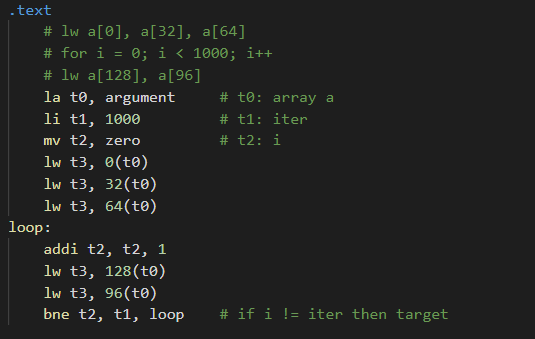
\includegraphics[width=8cm, height=6cm]{screenshot004}}
	\subfigure[LRU-LIP]{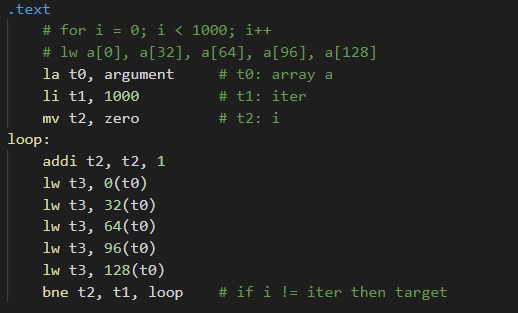
\includegraphics[width=8cm, height=6cm]{screenshot005}}
	\caption{Replacement Benchmarks}
	\label{fig:screenshot004}
\end{figure}

The first program will have better performance on LRU. In this example, LRU will keep a[96] and a[128] in cache, while LRU-LIP will evict them alternately (note that all five elements are hashed into the same set). Therefore, LRU very low miss rate while LRU-LIP have 100\% miss rate. In the second example, LRU-LIP has better performance. In this example, LRU will cyclically evict blocks from cache, causing all misses. LRU, on the contrary, only incurs two misses each iteration. Therefore, it has much lower miss rate. In actual design of a processor, we may prefer LRU if the programs running on top of it has very good temperal locality, i.e. elements visited will soon be revisited again. If considerable amounts of memory accesses are ramdom access that won't repeat itself, LRU-LIP may be a better choice.

\newpage
\resizebox{\textwidth}{10mm}{
	\begin{tabular}{|c|c|c|c|c|}
		\hline
		Replacement Policy & bench\_lru Miss Rate & bench\_lrulip Miss Rate & bench\_lru Total Cycles & bench\_lrulip Total Cycles \\
		\hline
		LRU & 0.25 & 100 & 10055 & 59006 \\
		\hline
		LRU-LIP & 100 & 40.06 & 26039 & 35030 \\
		\hline
	\end{tabular}
}


\subsection{Writehit Benchmarks}
\begin{figure}[h]
	\centering
	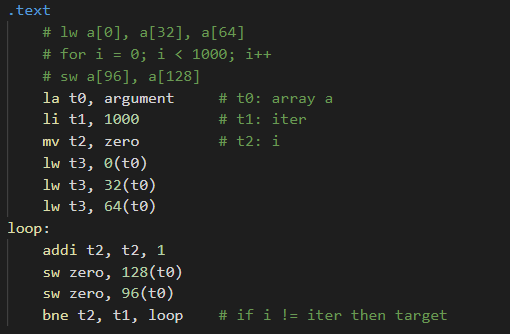
\includegraphics[width=8cm, height=6cm]{screenshot006}
	\caption{Writehit Benchmarks: Write-back}
	\label{fig:screenshot006}
\end{figure}

In bench\_writehit\_back, we repeated write to two blocks in cache. If we use write-back mode, no memory access will actually get to the main memory. However, if we use write-through mode, each and every access will be written back and cause a 10 cycle stall. However, since both modes don't affect cache state, they will have identical miss rate on every program. In this lab's settings, there is no way write-though will have better performance than write-back. This is because write-back only incurs a 10 cycle stall when eviction, while write-through, without help of write buffer, will stall on every access. In acutal implementation, write-through may be faster (with write buffer) and less expensive (no dirty bit).
\newline

\resizebox{\textwidth}{10mm}{
	\begin{tabular}{|c|c|c|c|c|}
		\hline
		Write Hit Policy & bench\_through Miss Rate & bench\_back Miss Rate & bench\_through Total Cycles & bench\_back Total Cycles \\
		\hline
		Write-back & N/A & 0.25 & N/A & 10055 \\
		\hline
		Write-through & N/A & 0.25 & N/A & 26039 \\
		\hline
	\end{tabular}
}

\newpage
\subsection{Writemiss Benchmarks}
\begin{figure}[h]
	\centering
	\subfigure[Allocate] {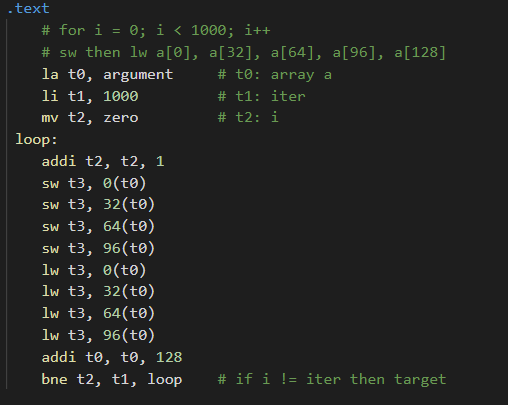
\includegraphics[width=8cm, height=6cm]{screenshot007}}
	\subfigure[No Allocate]{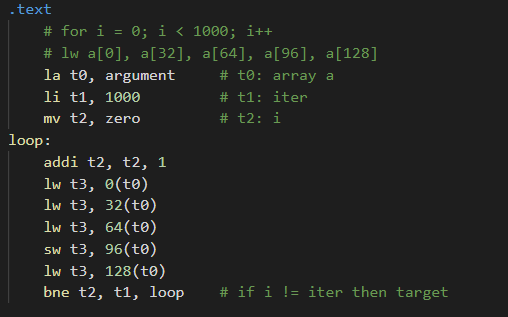
\includegraphics[width=8cm, height=6cm]{screenshot008}}
	\caption{Writemiss Benchmarks}
	\label{fig:screenshot007}
\end{figure}

In the first example, write-allocate will have better performance. If we allocate a block for each write, then in each iteration, only the four saves are miss. However, if we don't allocate, all eight operations will be miss. In the second example, no-write-allocate will have a better performance. If we allocate a block when saving 96(t0), cyclic eviction will happen, resulting in all misses. In actual design, if most write will be followed by a read, write-allocate is a good choice, o.w. we should use no-write-allocate.
\newline

\resizebox{\textwidth}{9mm}{
	\begin{tabular}{|c|c|c|c|c|}
		\hline
		Write Miss Ploicy & bench\_allocate Miss Rate & bench\_noallocate Miss Rate & bench\_allocate Total Cycles & bench\_noallocate Total Cycles \\
		\hline
		Write-allocate & 50 & 100 & 61006 & 60006 \\
		\hline
		No Write-allocate & 100 & 20.08 & 93006 & 28038 \\
		\hline
	\end{tabular}
}

\section{Ripes Bug Report}
Multiple ripes bugs are found during implementation. Listed as follows:

\noindent
\emph{1) Tag comparison failure } If we use skewed associative cache, blocks with same tag may be mapped into the same entry, no mechanism for detecting this. Solution: replace ALL tag comparison with address comparison.

\noindent
\emph{2) Cache bypassing } Cache is not used as a source of data. Therefore, if we randomly return data and report all accesses as hits, we can achieve low miss rate. Solution: no simple solution, suggest total rewrite of Ripes cache simulator.

\noindent
\emph{3) Revert failure } Revert function is only called upon reversion after a cache hit. Solution: modify caller.

\noindent
\emph{4) Wrong instra count } Different cache policies will have different instruction count on the same program. Solution: stall mechanism should be modified to support accurate instruction count.

\noindent
\emph{5) Cache statistics not available} Under rare circumstances (e.g. load after save etc.), hit and miss counter is dark. Solution: no simple solution, suggest a thorough check of cache simulator.

\noindent
\emph{6) Write-back not counted} After the program exits, cache content is not dumped to main memory, resulting in wrong writr-back count. Solution: add a dumping operation at the end of each run. 

\newpage
\section{Question Answering}
\noindent
\emph{1) By extracting useful patterns from large amounts of data, deep learning has produced
	dramatic breakthroughs in many areas. It is therefore natural to wonder if deep learning
	could help design better cache replacement policies since the replacement is also a
	prediction problem. Do you think deep learning, or other machine learning techniques, can
	be applied to cache replacement? What are the advantages and possible difficulties? If you
	are interested in this problem, you can further refer to this paper.}

From my perspective, deep learning may be used in cache replacement policies, but this will come with considerable difficulties. Sure enough, deep learning has good performance in pattern recognition and prediction. However, if we want to implement DNN using bare circuit, we may encounter the following problems: 1) DNN works on continuous numbers, while we only have 0/1 in circuits. How to make DNN accomodate to this setting is a big problem. 2) DNN is expensive to implement, we don't have room on chip for such a large module. 3) Cache replacement policy needs fast execution. DNN is rather slow in comparison with traditional algorithms. This requirement also makes impossible the idea of running DNN on a separate AI accelerator. 4) More complicated design is potentially more bug-prone. In lower levels of large systems, we always want to keep things simple. 5) DNN may have difficulty in transferring when the distribution changes. Traditional non-ML algorithms don't have this problem.
\newline

\noindent
\emph{2) In the lectures we discussed another optimization called non-blocking cache. Do you think it is useful in your processor? In your opinions how much is the cost and benefit?} 

I don't think it will be of any help in this processor. This processor has only one core and doesn't support OoO execution. This means that even if the cache per se is capable of responding to other accesses while pending on a miss, the processor won't be able to issue one. There is no benefit. Only the hardware cost and latency will increase.
\newline

\noindent
\emph{3) In the lectures we also discussed an optimization called software prefetching. For example,
	the RISC-V ISA can be extended to add a new prefetch offset(rs1) instruction. This
	instruction fetches the target block to the cache, but does not fill in any register yet.
	Therefore the actual load instruction executed later can be a cache hit. Obviously the
	compiler should insert this instruction at proper locations in the program, e.g., several
	instructions ahead of the actual loads to have enough time to prefetch. Do you think it is
	useful in your processor? In your opinions how much is the cost and benefit?}

Software prefetching will be quite useful in this processor. If the block needed is prefetched with appropriate timing, memory waiting stalls will be reduced to zero, although we need an extra instruciton for prefetching. The hardware cost is just some simple circuit. However, this will complicate the design of compilers a lot, resulting in much longer compiling time.

\end{document}